\documentclass[10pt,twocolumn,letterpaper]{article}

\usepackage{cvpr}
\usepackage{times}
\usepackage{epsfig}
\usepackage{graphicx}
\usepackage{amsmath}
\usepackage{amssymb}

% Include other packages here, before hyperref.

% If you comment hyperref and then uncomment it, you should delete
% egpaper.aux before re-running latex.  (Or just hit 'q' on the first latex
% run, let it finish, and you should be clear).
\usepackage[pagebackref=true,breaklinks=true,letterpaper=true,colorlinks,bookmarks=false]{hyperref}

%%%%%%%%% PAPER ID  - PLEASE UPDATE
\def\cvprPaperID{0446} % *** Enter the CVPR Paper ID here
\def\httilde{\mbox{\tt\raisebox{-.5ex}{\symbol{126}}}}

\begin{document}

%%%%%%%%% TITLE - PLEASE UPDATE
\title{Graph-Based Neural Reconstruction from Skeletonized 3D Networks}  % **** Enter the paper title here

\maketitle
\thispagestyle{empty}


%%%%%%%%% BODY TEXT - ENTER YOUR RESPONSE BELOW

We would like to thank the reviewers for their valuable feedback.

\subsection*{Reviewer 1}

\textbf{A1.} 
We thank the reviewer for pointing out four recent papers, and we will cite them in the next revision. However, we believe that our work focuses on a slightly different problem. Our algorithm corrects the split errors generated by current segmentation algorithms. These papers show impressive results but are fundamentally pixel-based methods, whereas our method explores higher level error correction. We take issue with the statement that ``the paper does not adequately reflect prior art, rendering its own conclusions questionable.'' In fact, reviewer 3 wrote ``the list of references is impressive, demonstrating comprehensive knowledge of both recent methods and the application domain.''

\textbf{A2.} 
This claim refers to building on-top of existing segmentation pipelines. We will clarify this point in our revision. In \textit{Learning to Agglomerate Superpixel Hierarchies}, Jain et al. extract a graph from superpixels generated by a watershed algorithm. We, on the other hand, use the output of \textit{LASH} as input to our framework.

\textbf{A3.} 
We do not agree with the statement that these are ``drastic'' errors, but rather honest mistakes. In fact, citing reference [18] for the multicut algorithm was done deliberately. We use the graph optimization library from Bjoern Andres' website\footnote{http://www.andres.sc/graph.html}, which cites [18] (his own work) for the multicut package. We will add an additional reference for U-Net that extends the original paper to 3D. We will update the reference to Funke et al.

\textbf{B1.} 
We agree that the skeletonization algorithm can be improved. Our goal for this paper was to use an existing method with its corresponding default parameters because it had been used previously for neuron skeletonization. We are currently working on an improved algorithm. 

\textbf{B2.} 
The skeletons shown are from an anisotropic dataset.

\textbf{B3.} 
The cubic region of interest is measured in nanometers, not voxels. We further discuss this parameter in the supplemental materials (Sec. 2.1). From section 4.8, ``Since our CNN only takes as input a region of the label volume we can train on anisotropic data and test on isotropic data.'' In the same section we show the results when training on isotropic data (Fig. 9). We will clarify this in the revision.


\textbf{B4.} 
We address this in the supplemental material, and we will reference it in the revision. 

\textbf{B5.} 
Without relying on the raw images we avoid retraining for every new dataset that has different staining or resolution. This reduces the amount of expert-labeled ground truth required for training every new dataset. In our opinion this is a big advantage. We will clarify this in the revision.

\textbf{B6.} 
This analysis is provided in Sec. 4.7 and Table 2.

\textbf{B7.} 
We are not using the lifted multicut.

\textbf{B8.}
The multicut algorithm does not enforce acyclic graphs but rather closed-surfaces and consistent solutions. We will update this in the next revision. We are currently working on adding additional domain-specific constraints.

\textbf{B9.} 
We mention the possibility for adding additional constraints to our framework in the future. We will clarify this in the revision.

\textbf{C1.} 
We use NeuroProof because it scales to terabyte datasets. Flood filling networks provide better accuracy but are much slower and work on a single neuron at a time. For dense reconstruction, NeuroProof is state-of-the-art. Variation of Information overcomes previous limitations of Rand error~\cite{lee2017superhuman,nunez2013machine}.

\textbf{C2.} 
Most of the current state-of-the-art methods are too slow to run on very large datasets, although we will compare against other baselines in the revision.

\subsection*{Reviewer 2}

The challenge datasets are generally too small for meaningful improvements. The datasets presented in our paper are ten times the size of these challenge datasets, and our method scales to much larger data. In a future revision, we will show the results of our network on these datasets.

\subsection*{Reviewer 3}


\begin{center}
	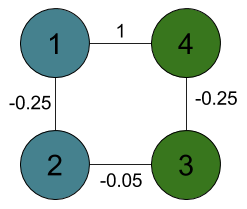
\includegraphics[width=0.28\linewidth]{./figures/MSF.png}
\end{center}


The figure above addresses one problem of using a minimum spanning forest, where negative and positive edges represent high and low affinities respectively. With a multicut formulation, the edge between nodes 1 and 4 will keep the blue and green segments separate. In a minimum spanning forest, nodes 1 and 4 will connect because of the moderate affinity between nodes 2 and 3.

{\small
\bibliographystyle{ieee}
\bibliography{egbib}
}

\end{document}
